% Options for packages loaded elsewhere
\PassOptionsToPackage{unicode}{hyperref}
\PassOptionsToPackage{hyphens}{url}
%
\documentclass[
]{book}
\usepackage{amsmath,amssymb}
\usepackage{lmodern}
\usepackage{ifxetex,ifluatex}
\ifnum 0\ifxetex 1\fi\ifluatex 1\fi=0 % if pdftex
  \usepackage[T1]{fontenc}
  \usepackage[utf8]{inputenc}
  \usepackage{textcomp} % provide euro and other symbols
\else % if luatex or xetex
  \usepackage{unicode-math}
  \defaultfontfeatures{Scale=MatchLowercase}
  \defaultfontfeatures[\rmfamily]{Ligatures=TeX,Scale=1}
\fi
% Use upquote if available, for straight quotes in verbatim environments
\IfFileExists{upquote.sty}{\usepackage{upquote}}{}
\IfFileExists{microtype.sty}{% use microtype if available
  \usepackage[]{microtype}
  \UseMicrotypeSet[protrusion]{basicmath} % disable protrusion for tt fonts
}{}
\makeatletter
\@ifundefined{KOMAClassName}{% if non-KOMA class
  \IfFileExists{parskip.sty}{%
    \usepackage{parskip}
  }{% else
    \setlength{\parindent}{0pt}
    \setlength{\parskip}{6pt plus 2pt minus 1pt}}
}{% if KOMA class
  \KOMAoptions{parskip=half}}
\makeatother
\usepackage{xcolor}
\IfFileExists{xurl.sty}{\usepackage{xurl}}{} % add URL line breaks if available
\IfFileExists{bookmark.sty}{\usepackage{bookmark}}{\usepackage{hyperref}}
\hypersetup{
  pdftitle={Statistics Labs for Psychology},
  pdfauthor={Zakary A. Draper},
  hidelinks,
  pdfcreator={LaTeX via pandoc}}
\urlstyle{same} % disable monospaced font for URLs
\usepackage{color}
\usepackage{fancyvrb}
\newcommand{\VerbBar}{|}
\newcommand{\VERB}{\Verb[commandchars=\\\{\}]}
\DefineVerbatimEnvironment{Highlighting}{Verbatim}{commandchars=\\\{\}}
% Add ',fontsize=\small' for more characters per line
\usepackage{framed}
\definecolor{shadecolor}{RGB}{248,248,248}
\newenvironment{Shaded}{\begin{snugshade}}{\end{snugshade}}
\newcommand{\AlertTok}[1]{\textcolor[rgb]{0.94,0.16,0.16}{#1}}
\newcommand{\AnnotationTok}[1]{\textcolor[rgb]{0.56,0.35,0.01}{\textbf{\textit{#1}}}}
\newcommand{\AttributeTok}[1]{\textcolor[rgb]{0.77,0.63,0.00}{#1}}
\newcommand{\BaseNTok}[1]{\textcolor[rgb]{0.00,0.00,0.81}{#1}}
\newcommand{\BuiltInTok}[1]{#1}
\newcommand{\CharTok}[1]{\textcolor[rgb]{0.31,0.60,0.02}{#1}}
\newcommand{\CommentTok}[1]{\textcolor[rgb]{0.56,0.35,0.01}{\textit{#1}}}
\newcommand{\CommentVarTok}[1]{\textcolor[rgb]{0.56,0.35,0.01}{\textbf{\textit{#1}}}}
\newcommand{\ConstantTok}[1]{\textcolor[rgb]{0.00,0.00,0.00}{#1}}
\newcommand{\ControlFlowTok}[1]{\textcolor[rgb]{0.13,0.29,0.53}{\textbf{#1}}}
\newcommand{\DataTypeTok}[1]{\textcolor[rgb]{0.13,0.29,0.53}{#1}}
\newcommand{\DecValTok}[1]{\textcolor[rgb]{0.00,0.00,0.81}{#1}}
\newcommand{\DocumentationTok}[1]{\textcolor[rgb]{0.56,0.35,0.01}{\textbf{\textit{#1}}}}
\newcommand{\ErrorTok}[1]{\textcolor[rgb]{0.64,0.00,0.00}{\textbf{#1}}}
\newcommand{\ExtensionTok}[1]{#1}
\newcommand{\FloatTok}[1]{\textcolor[rgb]{0.00,0.00,0.81}{#1}}
\newcommand{\FunctionTok}[1]{\textcolor[rgb]{0.00,0.00,0.00}{#1}}
\newcommand{\ImportTok}[1]{#1}
\newcommand{\InformationTok}[1]{\textcolor[rgb]{0.56,0.35,0.01}{\textbf{\textit{#1}}}}
\newcommand{\KeywordTok}[1]{\textcolor[rgb]{0.13,0.29,0.53}{\textbf{#1}}}
\newcommand{\NormalTok}[1]{#1}
\newcommand{\OperatorTok}[1]{\textcolor[rgb]{0.81,0.36,0.00}{\textbf{#1}}}
\newcommand{\OtherTok}[1]{\textcolor[rgb]{0.56,0.35,0.01}{#1}}
\newcommand{\PreprocessorTok}[1]{\textcolor[rgb]{0.56,0.35,0.01}{\textit{#1}}}
\newcommand{\RegionMarkerTok}[1]{#1}
\newcommand{\SpecialCharTok}[1]{\textcolor[rgb]{0.00,0.00,0.00}{#1}}
\newcommand{\SpecialStringTok}[1]{\textcolor[rgb]{0.31,0.60,0.02}{#1}}
\newcommand{\StringTok}[1]{\textcolor[rgb]{0.31,0.60,0.02}{#1}}
\newcommand{\VariableTok}[1]{\textcolor[rgb]{0.00,0.00,0.00}{#1}}
\newcommand{\VerbatimStringTok}[1]{\textcolor[rgb]{0.31,0.60,0.02}{#1}}
\newcommand{\WarningTok}[1]{\textcolor[rgb]{0.56,0.35,0.01}{\textbf{\textit{#1}}}}
\usepackage{longtable,booktabs,array}
\usepackage{calc} % for calculating minipage widths
% Correct order of tables after \paragraph or \subparagraph
\usepackage{etoolbox}
\makeatletter
\patchcmd\longtable{\par}{\if@noskipsec\mbox{}\fi\par}{}{}
\makeatother
% Allow footnotes in longtable head/foot
\IfFileExists{footnotehyper.sty}{\usepackage{footnotehyper}}{\usepackage{footnote}}
\makesavenoteenv{longtable}
\usepackage{graphicx}
\makeatletter
\def\maxwidth{\ifdim\Gin@nat@width>\linewidth\linewidth\else\Gin@nat@width\fi}
\def\maxheight{\ifdim\Gin@nat@height>\textheight\textheight\else\Gin@nat@height\fi}
\makeatother
% Scale images if necessary, so that they will not overflow the page
% margins by default, and it is still possible to overwrite the defaults
% using explicit options in \includegraphics[width, height, ...]{}
\setkeys{Gin}{width=\maxwidth,height=\maxheight,keepaspectratio}
% Set default figure placement to htbp
\makeatletter
\def\fps@figure{htbp}
\makeatother
\setlength{\emergencystretch}{3em} % prevent overfull lines
\providecommand{\tightlist}{%
  \setlength{\itemsep}{0pt}\setlength{\parskip}{0pt}}
\setcounter{secnumdepth}{5}
\usepackage{booktabs}
\usepackage{amsthm}
\makeatletter
\def\thm@space@setup{%
  \thm@preskip=8pt plus 2pt minus 4pt
  \thm@postskip=\thm@preskip
}
\makeatother
\ifluatex
  \usepackage{selnolig}  % disable illegal ligatures
\fi
\usepackage[]{natbib}
\bibliographystyle{apalike}

\title{Statistics Labs for Psychology}
\author{Zakary A. Draper}
\date{2021-09-27}

\begin{document}
\maketitle

{
\setcounter{tocdepth}{1}
\tableofcontents
}
\hypertarget{lab-outline}{%
\chapter*{Lab Outline}\label{lab-outline}}
\addcontentsline{toc}{chapter}{Lab Outline}

\hypertarget{summary}{%
\section*{Summary}\label{summary}}
\addcontentsline{toc}{section}{Summary}

The lab component of this course primarily concerns statistical methods and analysis, and of course the use of computer programs. The universe of statistical models is extraordinarily vast. We will focus on common statistical tests that can be broadly classified as linear models. Students will learn to model a diverse array of hypotheses as linear models.

\hypertarget{learning-outcomes}{%
\section*{Learning Outcomes}\label{learning-outcomes}}
\addcontentsline{toc}{section}{Learning Outcomes}

At the conclusion of this course, students will be able to:

\begin{enumerate}
\def\labelenumi{\arabic{enumi}.}
\tightlist
\item
  Appropriately evaluate the strength of evidence provided by common statistical tests conducted using a linear regression framework.
\item
  Conduct common statistical tests in R.
\item
  Produce informative, aesthetically pleasing, data visualizations, in accordance with APA style guidelines.
\item
  Utilize online resources to expand their knowledge related to outcomes 1--3, such that they will be able to understand and appropriately utilize statistical concepts that are not taught in this course.
\end{enumerate}

\hypertarget{software}{%
\section*{Software}\label{software}}
\addcontentsline{toc}{section}{Software}

\hypertarget{r}{%
\subsection*{\texorpdfstring{\href{https://www.r-project.org/}{R}}{R}}\label{r}}
\addcontentsline{toc}{subsection}{\href{https://www.r-project.org/}{R}}

R refers to both a programming language for statistical computing and software. It is a free and open source project. We will be doing all of our data analysis using the R programming language.

\hypertarget{rstudio}{%
\subsection*{\texorpdfstring{\href{https://rstudio.com/}{RStudio}}{RStudio}}\label{rstudio}}
\addcontentsline{toc}{subsection}{\href{https://rstudio.com/}{RStudio}}

RStudio is a commercial organization that offers a free and open source version of desktop software. The RStudio desktop software is an integrated development environment. Which is to say, it is software for executing R code. RStudio has several benefits over the base R software.

\hypertarget{syzygy-optional}{%
\subsection*{\texorpdfstring{\href{https://ubc.syzygy.ca/}{Syzygy} (Optional)}{Syzygy (Optional)}}\label{syzygy-optional}}
\addcontentsline{toc}{subsection}{\href{https://ubc.syzygy.ca/}{Syzygy} (Optional)}

The R and RStudio software are available for Windows, Mac, and Linux operating systems. Neither will operate on a tablet or Chromebook. If you are using a tablet or Chromebook, you can run R in a web browser using a web application called Jupyter Notebook. A Jupyter Notebook that has been set up to run R is available to UBCO students at \url{https://ubc.syzygy.ca/}. You can sign in to Syzygy with your CWL.

Jupyter Notebook is an entirely separate interface from RStudio. The R code is the same, but the interface is difference. We recommend using RStudio if possible, not because it is better, but because it is what we will be using. However, if RStudio is unavailable to you, or you just want to use Juptyer, then you should feel empowered to do so. You can absolutely be successful in this course using Jupyter.

\hypertarget{xquartz}{%
\subsection*{\texorpdfstring{\href{https://www.xquartz.org/}{XQuartz}}{XQuartz}}\label{xquartz}}
\addcontentsline{toc}{subsection}{\href{https://www.xquartz.org/}{XQuartz}}

If you are using a Mac, you will need to install XQuartz. XQuartz is required to install some of the R packages we will make frequent use of throughout the course. It is free and open source.

\hypertarget{zoom}{%
\subsection*{Zoom}\label{zoom}}
\addcontentsline{toc}{subsection}{Zoom}

Office hours with the lab instructors will be held via Zoom.

\hypertarget{canvas}{%
\subsection*{Canvas}\label{canvas}}
\addcontentsline{toc}{subsection}{Canvas}

We will use Canvas to share information and documents, including data sets, slides, and other useful materials.

\hypertarget{evaluation}{%
\section*{Evaluation}\label{evaluation}}
\addcontentsline{toc}{section}{Evaluation}

The lab will be worth 30\% of your final grade, divided across lab reports (21\%), and quizzes (9\%).

\hypertarget{lab-reports-21}{%
\subsection*{Lab Reports (21\%)}\label{lab-reports-21}}
\addcontentsline{toc}{subsection}{Lab Reports (21\%)}

Lab reports are brief, APA-style manuscripts, reporting and discussing the results of a study. You will receive 21\% of your grade for completing 3 lab reports, each of which is worth 7\% of your final grade. For each lab report, you will be provided with preregistration information for a hypothetical study as well as simulated data from that study. You will be responsible for writing the results and discussion, creating an appropriate data visualization, and preparing a reproducible R script, which will be submitted with the report. Specific instructions for each lab are provided in the lab manual.

You may choose to complete lab reports on any of the statistical tests covered in the lab manual. Lab reports for a given lab are due the Monday following the lab at 11:59 PM. Late lab reports will not be accepted. Lab reports will be marked and returned with detailed feedback by the beginning of the next week's lab.

Optionally, you may submit a 4th lab report. If you do, your final lab report grade will be based on the best 3 of the 4 labs you submit.

\hypertarget{quizzes-9}{%
\subsection*{Quizzes (9\%)}\label{quizzes-9}}
\addcontentsline{toc}{subsection}{Quizzes (9\%)}

There are two quizzes. The first is worth 3\% of your final grade. It will cover R fundamentals that you will need to master to be successful in this course (and in 373). The second and final quiz is worth 6\% of your final grade. It will take the form of a lab report that is completed during regular lab time.

\hypertarget{tentative-schedule}{%
\section*{Tentative Schedule}\label{tentative-schedule}}
\addcontentsline{toc}{section}{Tentative Schedule}

As indicated by the title of this section. This schedule is tentative and therefore subject may change. These are the topics we plan to cover, in the order we expect to cover them.

Labs 1--2 will cover the fundamentals of R and RStudio. Lab 3 will introduce you to data visualization using \texttt{ggplot2}. The next lab will be a quiz that will require practical application of the skills you learn in labs 1--3.

Beginning in week 6, each lab will cover one statistical test. For each of these statistical tests, you will be presented with preregistered information from a hypothetical study. Most of these studies are based on real research programs (many of which are being actively investigated by researchers at UBCO!). If the content of one of the labs interests you, consider reaching out to the professor whose research inspired it. There may be opportunities to work with that professor on a directed studies or honours project.

\begin{longtable}[]{@{}cll@{}}
\toprule
Week & Date & Topic \\
\midrule
\endhead
1 & Sep.~09 & Introduction to R \\
2 & Sep.~16 & Introduction to R, part 2 \\
3 & Sep.~23 & Data visualisation with ggplot2 \\
4 & Sep.~30 & National Day for Truth and Reconciliation. No Lab. \\
5 & Oct.~07 & Quiz 1 \\
5 & Oct.~14 & One sample \emph{t} test \\
6 & Oct.~21 & Paired samples \emph{t} test \\
7 & Oct.~28 & Independent samples \emph{t} test \\
8 & Nov.~04 & Correlation \\
10 & Nov.~11 & Midterm Break \\
11 & Nov.~18 & ANOVA \\
12 & Nov.~25 & Factorial ANOVA \\
13 & Dec.~02 & Final Quiz \\
\bottomrule
\end{longtable}

\hypertarget{intro1}{%
\chapter{Introduction to R}\label{intro1}}

\hypertarget{learning-objectives}{%
\section{Learning Objectives}\label{learning-objectives}}

After completing this lab, you should be able to:

\begin{itemize}
\tightlist
\item
  Explain what R is and describe its main uses.
\item
  Give (at least) 3 benefits of using R for data analysis.
\item
  Create R objects.
\item
  Identify R objects of the following R classes: numeric, character, logical, data.frame.
\item
  Apply basic operations to vectors in R.
\item
  Explain the basic structure of function calls.
\item
  Write scripts to manually enter data as \texttt{data.frame}s in R.
\end{itemize}

\hypertarget{prepare-for-the-lab}{%
\section{Prepare for the Lab}\label{prepare-for-the-lab}}

Before coming to the lab, install R and RStudio on your computer. There are computers in the lab with R and RStudio installed, so if you are planning to use the lab computers for the semester, then you do not need to install

\hypertarget{install-r}{%
\subsection{Install R}\label{install-r}}

You can find links for downloading R and other information about R on the R website \url{https://www.r-project.org}. You can download R from one of several CRAN mirrors. The simplest option is the cloud (\url{https://cloud.r-project.org/}), which will automatically redirect you to a local server.

\hypertarget{install-rstudio}{%
\subsection{Install RStudio}\label{install-rstudio}}

Download and install the desktop version of RStudio from \url{https://rstudio.com/products/rstudio/}.

\hypertarget{im-using-a-tablet-or-chromebook}{%
\subsection{I'm Using a Tablet or Chromebook}\label{im-using-a-tablet-or-chromebook}}

You cannot install R or RStudio to these devices. You can run R using a Jupyter Notebook. The simplest way to make this happen is going to \url{https://ubc.syzygy.ca/} in your web browser and logging in with your CWL. Make sure you are able to sign in to this before the lab.

\hypertarget{can-i-use-a-lab-computer}{%
\subsection{Can I Use a Lab Computer?}\label{can-i-use-a-lab-computer}}

Yes. There are computers in the room where we will be holding the lab that have R installed already. If you are planning to use the lab computers for the entire semester, you are welcome to do so. Just know that will likely become fairly annoying when you have to work on lab work outside of regular lab hours (or if you are unable to attend the lab for some reason). Even if you plan on primarily using the lab computers, we recommend having a personal machine that you can use for doing your lab work.

If you do plan to use the lab computers, visit the lab room before the lab and ensure that you are able to sign in to the computers. We will not be able to take time out of the lab to provide support with logging into the campus machines.

\hypertarget{lab-activity}{%
\section{Lab Activity}\label{lab-activity}}

\hypertarget{mathematical-operations}{%
\subsection{Mathematical Operations}\label{mathematical-operations}}

Write R code to solve each of these equations:

\begin{enumerate}
\def\labelenumi{\arabic{enumi}.}
\tightlist
\item
  \(1/20\)
\item
  \(\frac{1}{20 \times 20}\)
\item
  \(1 - .95^{10}\)
\item
  \(\sqrt{19}\)
\end{enumerate}

\hypertarget{object-assignment}{%
\subsection{Object Assignment}\label{object-assignment}}

Use the assignment operator, \texttt{\textless{}-}, to define R objects with the names and values shown in the table below.

\begin{longtable}[]{@{}ll@{}}
\toprule
name & value \\
\midrule
\endhead
x & 10 \\
y & 4.2 \\
haiku & a haiku about R \\
excited & logical, honest answer to the question, ``I am excited to learn R'' \\
\bottomrule
\end{longtable}

\hypertarget{object-classes}{%
\subsection{Object Classes}\label{object-classes}}

Use \texttt{class()} to identify the class(es) of each of the objects you just created.

\hypertarget{longer-vectors}{%
\subsection{Longer Vectors}\label{longer-vectors}}

A vector is a list of items of the same type. Vectors can contain numbers, characters, or logicals, so long as every item in that vector is the same class. The objects you have created thus far are all vectors of length one. That is, they each contain one item. But vectors more often contain many items.

You can combine items into a vector using \texttt{c()}, which is the concatenate/combine function. This function takes any number of arguments, each separated by a comma, and combines them into a vector.

Use the assignment operator, \texttt{\textless{}-}, and the concatenate function, \texttt{c()} to define R objects with the names and values shown in the table below.

\begin{longtable}[]{@{}ll@{}}
\toprule
name & value \\
\midrule
\endhead
dub & a numeric/double vector of length 3 \\
dub2 & a numeric/double vector of length 4 \\
\bottomrule
\end{longtable}

You can also name elements in your vector, as in the example below.

\begin{Shaded}
\begin{Highlighting}[]
\NormalTok{ages }\OtherTok{\textless{}{-}} \FunctionTok{c}\NormalTok{(}\StringTok{"Declan"} \OtherTok{=} \DecValTok{17}\NormalTok{, }\StringTok{"Ava"} \OtherTok{=} \DecValTok{19}\NormalTok{, }\StringTok{"Liam"} \OtherTok{=} \DecValTok{20}\NormalTok{, }\StringTok{"Charlotte"} \OtherTok{=} \DecValTok{19}\NormalTok{)}
\end{Highlighting}
\end{Shaded}

For longer function calls, it is easier to read if they are spread out over several lines. The code below is formatted differently, but functionally identical to the code which used only one line.

\begin{Shaded}
\begin{Highlighting}[]
\NormalTok{ages }\OtherTok{\textless{}{-}} \FunctionTok{c}\NormalTok{(}
  \StringTok{"Declan"} \OtherTok{=} \DecValTok{17}\NormalTok{,}
  \StringTok{"Ava"} \OtherTok{=} \DecValTok{19}\NormalTok{,}
  \StringTok{"Liam"} \OtherTok{=} \DecValTok{20}\NormalTok{,}
  \StringTok{"Charlotte"} \OtherTok{=} \DecValTok{19}
\NormalTok{)}
\end{Highlighting}
\end{Shaded}

\begin{Shaded}
\begin{Highlighting}[]
\NormalTok{ages}
\end{Highlighting}
\end{Shaded}

\begin{verbatim}
##    Declan       Ava      Liam Charlotte 
##        17        19        20        19
\end{verbatim}

This can be useful, but a more common approach is to use data frames.

\hypertarget{data-frames}{%
\subsection{Data Frames}\label{data-frames}}

A \texttt{data.frame} is a special class of R object that groups vectors into columns. This is a useful way of organizing and presenting data. It is easy to read and understand. The data we will work with this semester will be organized in a \texttt{data.frame}.

Create a \texttt{data.frame} using the function \texttt{data.frame()}. Like \texttt{c()}, \texttt{data.frame()}, combines its arguments. However, instead of combining elements into a vectors, \texttt{data.frame()} binds vectors into columns of a table.

\begin{Shaded}
\begin{Highlighting}[]
\FunctionTok{data.frame}\NormalTok{(}
  \AttributeTok{name =} \FunctionTok{c}\NormalTok{(}\StringTok{"Declan"}\NormalTok{, }\StringTok{"Ava"}\NormalTok{, }\StringTok{"Liam"}\NormalTok{, }\StringTok{"Charlotte"}\NormalTok{),}
  \AttributeTok{age =} \FunctionTok{c}\NormalTok{(}\DecValTok{17}\NormalTok{, }\DecValTok{19}\NormalTok{, }\DecValTok{20}\NormalTok{, }\DecValTok{19}\NormalTok{)}
\NormalTok{)}
\end{Highlighting}
\end{Shaded}

\begin{verbatim}
##        name age
## 1    Declan  17
## 2       Ava  19
## 3      Liam  20
## 4 Charlotte  19
\end{verbatim}

This \texttt{data.frame} has the same information as the vector \texttt{ages} we created previously. Except the information is stored in two vectors---\texttt{name} and \texttt{age}---instead of one named vector. The ability to store information this way becomes increasingly useful if we want to more information about these individuals, as in the example below.

Recreate the following in R. Save the result as an object named \texttt{happiness}.

\begin{verbatim}
##        name age group shs_1 shs_2 shs_3
## 1    Declan  17     A     3     4     4
## 2       Ava  19     A     4     3     3
## 3      Liam  20     B     5     5     4
## 4 Charlotte  19     B     4     5     5
\end{verbatim}

\hypertarget{add-a-column-to-a-data-frame}{%
\subsection{Add a Column to a Data Frame}\label{add-a-column-to-a-data-frame}}

Use \texttt{\$} to add a column called \texttt{shs\_total} to \texttt{happiness}, which is the sum of \texttt{shs\_1}, \texttt{shs\_2}, and \texttt{shs\_3}. The result should look like this.

\begin{verbatim}
##        name age group shs_1 shs_2 shs_3 shs_total
## 1    Declan  17     A     3     4     4        11
## 2       Ava  19     A     4     3     3        10
## 3      Liam  20     B     5     5     4        14
## 4 Charlotte  19     B     4     5     5        14
\end{verbatim}

\hypertarget{summary-statistics}{%
\subsection{Summary Statistics}\label{summary-statistics}}

Use R functions to compute the mean, median, and standard deviation of \texttt{shs\_total}.

\hypertarget{discussion-questions}{%
\section{Discussion Questions}\label{discussion-questions}}

Be prepared to answer the following questions. It is okay (even good!) to use R to discover the answers to these questions.

\begin{enumerate}
\def\labelenumi{\arabic{enumi}.}
\tightlist
\item
  What is the class of \texttt{happiness}? Why does it make sense to store data using objects of this class?
\item
  What is the class of \texttt{happiness\$shs\_tot}?
\item
  Why is the \texttt{\$} needed to reference columns in a \texttt{data.frame}?
\item
  What is the output of \texttt{happiness\$shs\_tot\ +\ 2}?
\item
  What class is the object produced by executing: \texttt{c(happiness\$shs\_tot,\ happiness\$group)}?
\item
  What is the difference between \texttt{1} and \texttt{"1"} in R?
\item
  Why does \texttt{Happiness\$shs\_tot\ +\ 2} return an error?
\end{enumerate}

\hypertarget{resources}{%
\section{Resources}\label{resources}}

\href{assets/slides/01-intro-to-r-1-slides.pdf}{Slides}

\hypertarget{intro2}{%
\chapter{Introduction to R (Part 2)}\label{intro2}}

\begin{figure}
\centering
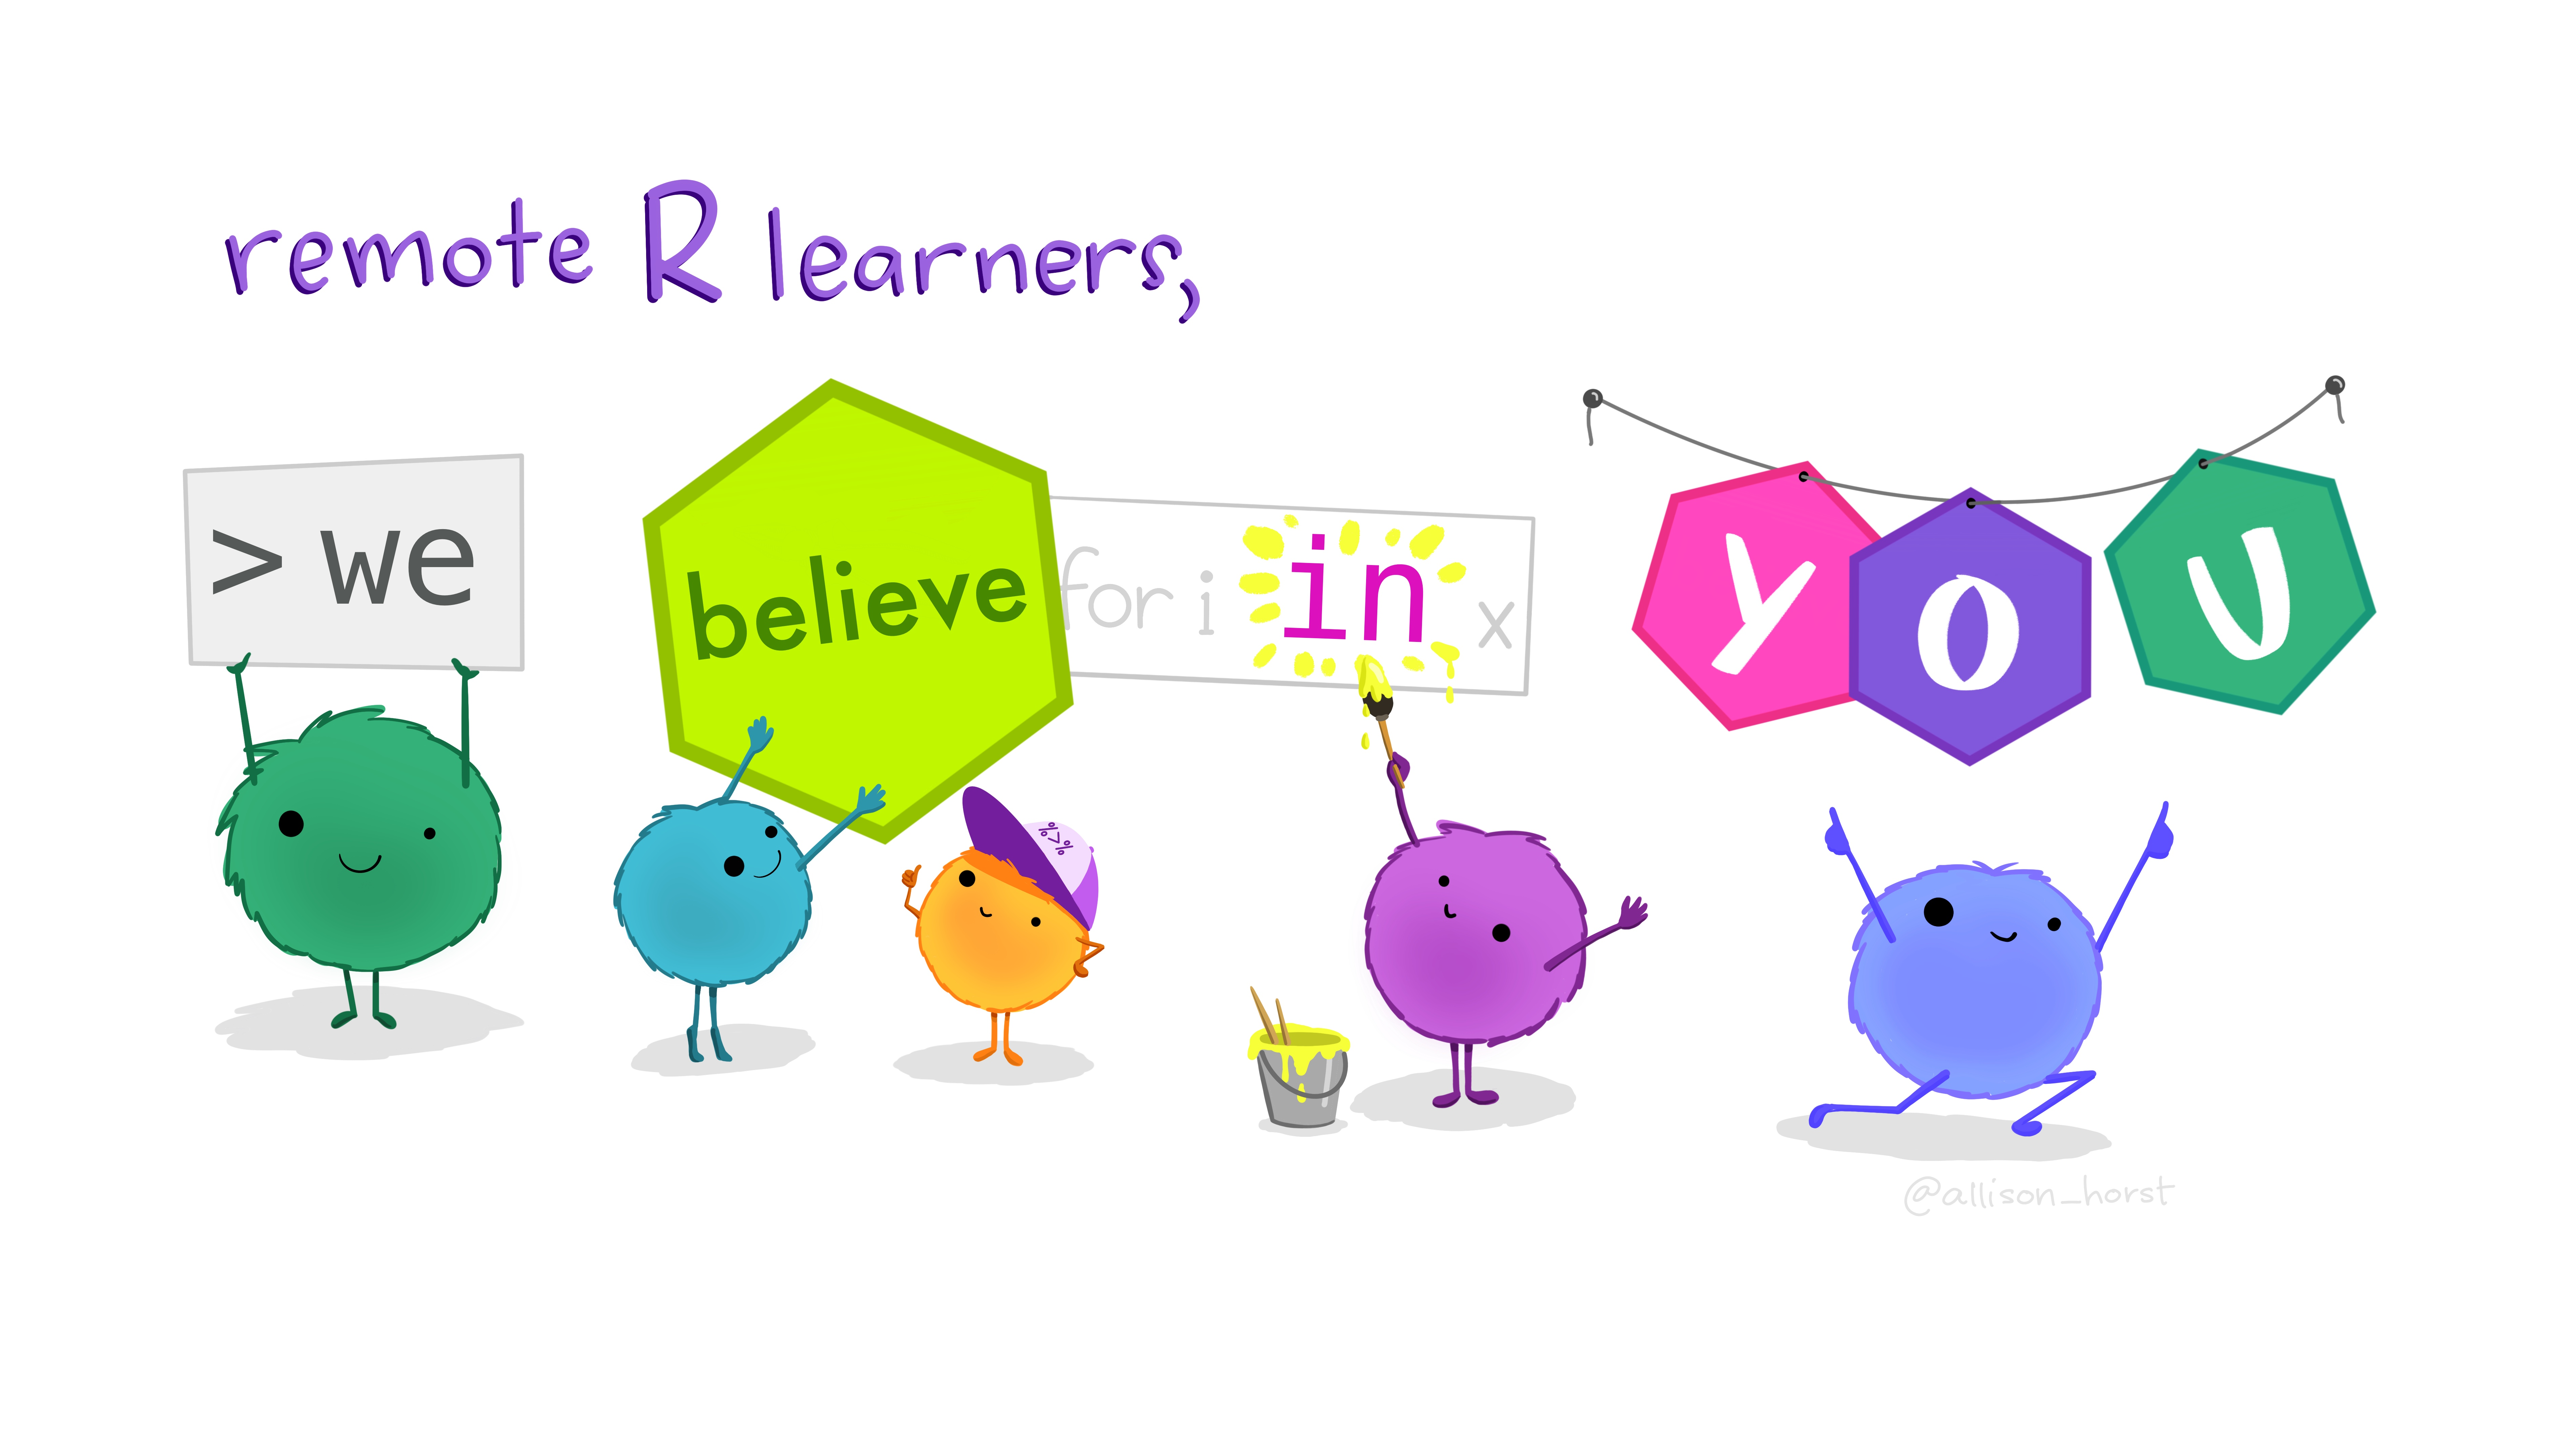
\includegraphics{assets/images/monster_support.jpg}
\caption{We believe in you!}
\end{figure}

\hypertarget{learning-objectives-1}{%
\section{Learning Objectives}\label{learning-objectives-1}}

After completing this lab, you should be able to:

\begin{itemize}
\tightlist
\item
  Reference files using absolute and relative paths.
\item
  Create an R data frame from a data file stored on your computer.
\item
  Convert numeric or character vectors to factors.
\item
  Index vectors and data frames.
\end{itemize}

\hypertarget{prepare-for-the-lab-1}{%
\section{Prepare for the Lab}\label{prepare-for-the-lab-1}}

\begin{itemize}
\tightlist
\item
  Make sure you grasp the concepts from lab 1.
\item
  Read \href{https://r4ds.had.co.nz/workflow-projects.html}{Workflow: projects} from \href{https://r4ds.had.co.nz/}{R for Data Science}.
\item
  Read the following sections from \href{https://learningstatisticswithr.com/}{Learning Statistics with R}:

  \begin{itemize}
  \tightlist
  \item
    \href{https://learningstatisticswithr.com/book/mechanics.html\#useful}{4.6 Useful things to know about variables}
  \item
    \href{https://learningstatisticswithr.com/book/mechanics.html\#factors}{4.7 Factors}
  \end{itemize}
\end{itemize}

\hypertarget{lab-activity-1}{%
\section{Lab Activity}\label{lab-activity-1}}

Researchers at the Vancouver and Okanagan campuses of The University of British Columbia have conducted a survey of child sleep. The results of this survey are found in the file \href{assets/data/child-sleep-data.csv}{child-sleep-data.csv}. The table below provides names and descriptions for each variable in the data set.

Name

Description

id

A randomly generated participant ID, unique to each participant.

age

The age of the child in the study.

campus

The campus from which the participant was recruited (``Point Grey'' or ``Okanagan'').

sleep\_location

Where does the child sleep? 1 = co-sleeps with parent(s); 2 = sleeps in own room; 3 = shares a room but does not cosleep.

sleep

The parent's estimate of the average hours of sleep the child receives in a 24-hour period.

Download \href{assets/data/child-sleep-data.csv}{child-sleep-data.csv} and then complete the following steps:

\hypertarget{import-and-inspect-the-data}{%
\subsection{Import and Inspect the Data}\label{import-and-inspect-the-data}}

\begin{itemize}
\tightlist
\item
  Import \href{assets/data/child-sleep-data.csv}{child-sleep-data.csv} into R; assign it a meaningful name.
\item
  Inspect the \texttt{data.frame} using \texttt{str()}, \texttt{head()}, and \texttt{View()}.
\end{itemize}

\hypertarget{convert-categorical-variables-to-factors}{%
\subsection{Convert Categorical Variables to Factors}\label{convert-categorical-variables-to-factors}}

\begin{itemize}
\tightlist
\item
  Use \texttt{as.factor()} and \texttt{factor()} to convert any categorical variables to factors with the appropriate levels and labels.
\end{itemize}

\hypertarget{subsetting-and-logical-expressions}{%
\subsection{Subsetting and Logical Expressions}\label{subsetting-and-logical-expressions}}

Use \texttt{{[}{]}} to subset the data frame and find the answers to following questions/complete the tasks described below. You will also need to use \texttt{is.na()}, \texttt{max()}, \texttt{min()}, \texttt{mean()}, and logical expressions.

\begin{itemize}
\tightlist
\item
  What campus was the 48th participant recruited at?
\item
  Return the data for participants who are missing responses on the sleep variable.
\item
  What proportion of participants are missing data for the sleep variable?
\item
  On average, how many hours do the children in this sample sleep per day?
\item
  What is the average daily sleep of children in each of the three conditions?
\item
  What is the participant ID of the participant(s) who reported the most sleep? The least sleep?
\end{itemize}

\hypertarget{participant-information}{%
\subsection{Participant Information}\label{participant-information}}

Use \texttt{table()} to identify how many, and what proportion of participants belong to each level of the three categorical variables.

\hypertarget{data-viz}{%
\chapter{Data Visualization}\label{data-viz}}

\begin{figure}
\centering
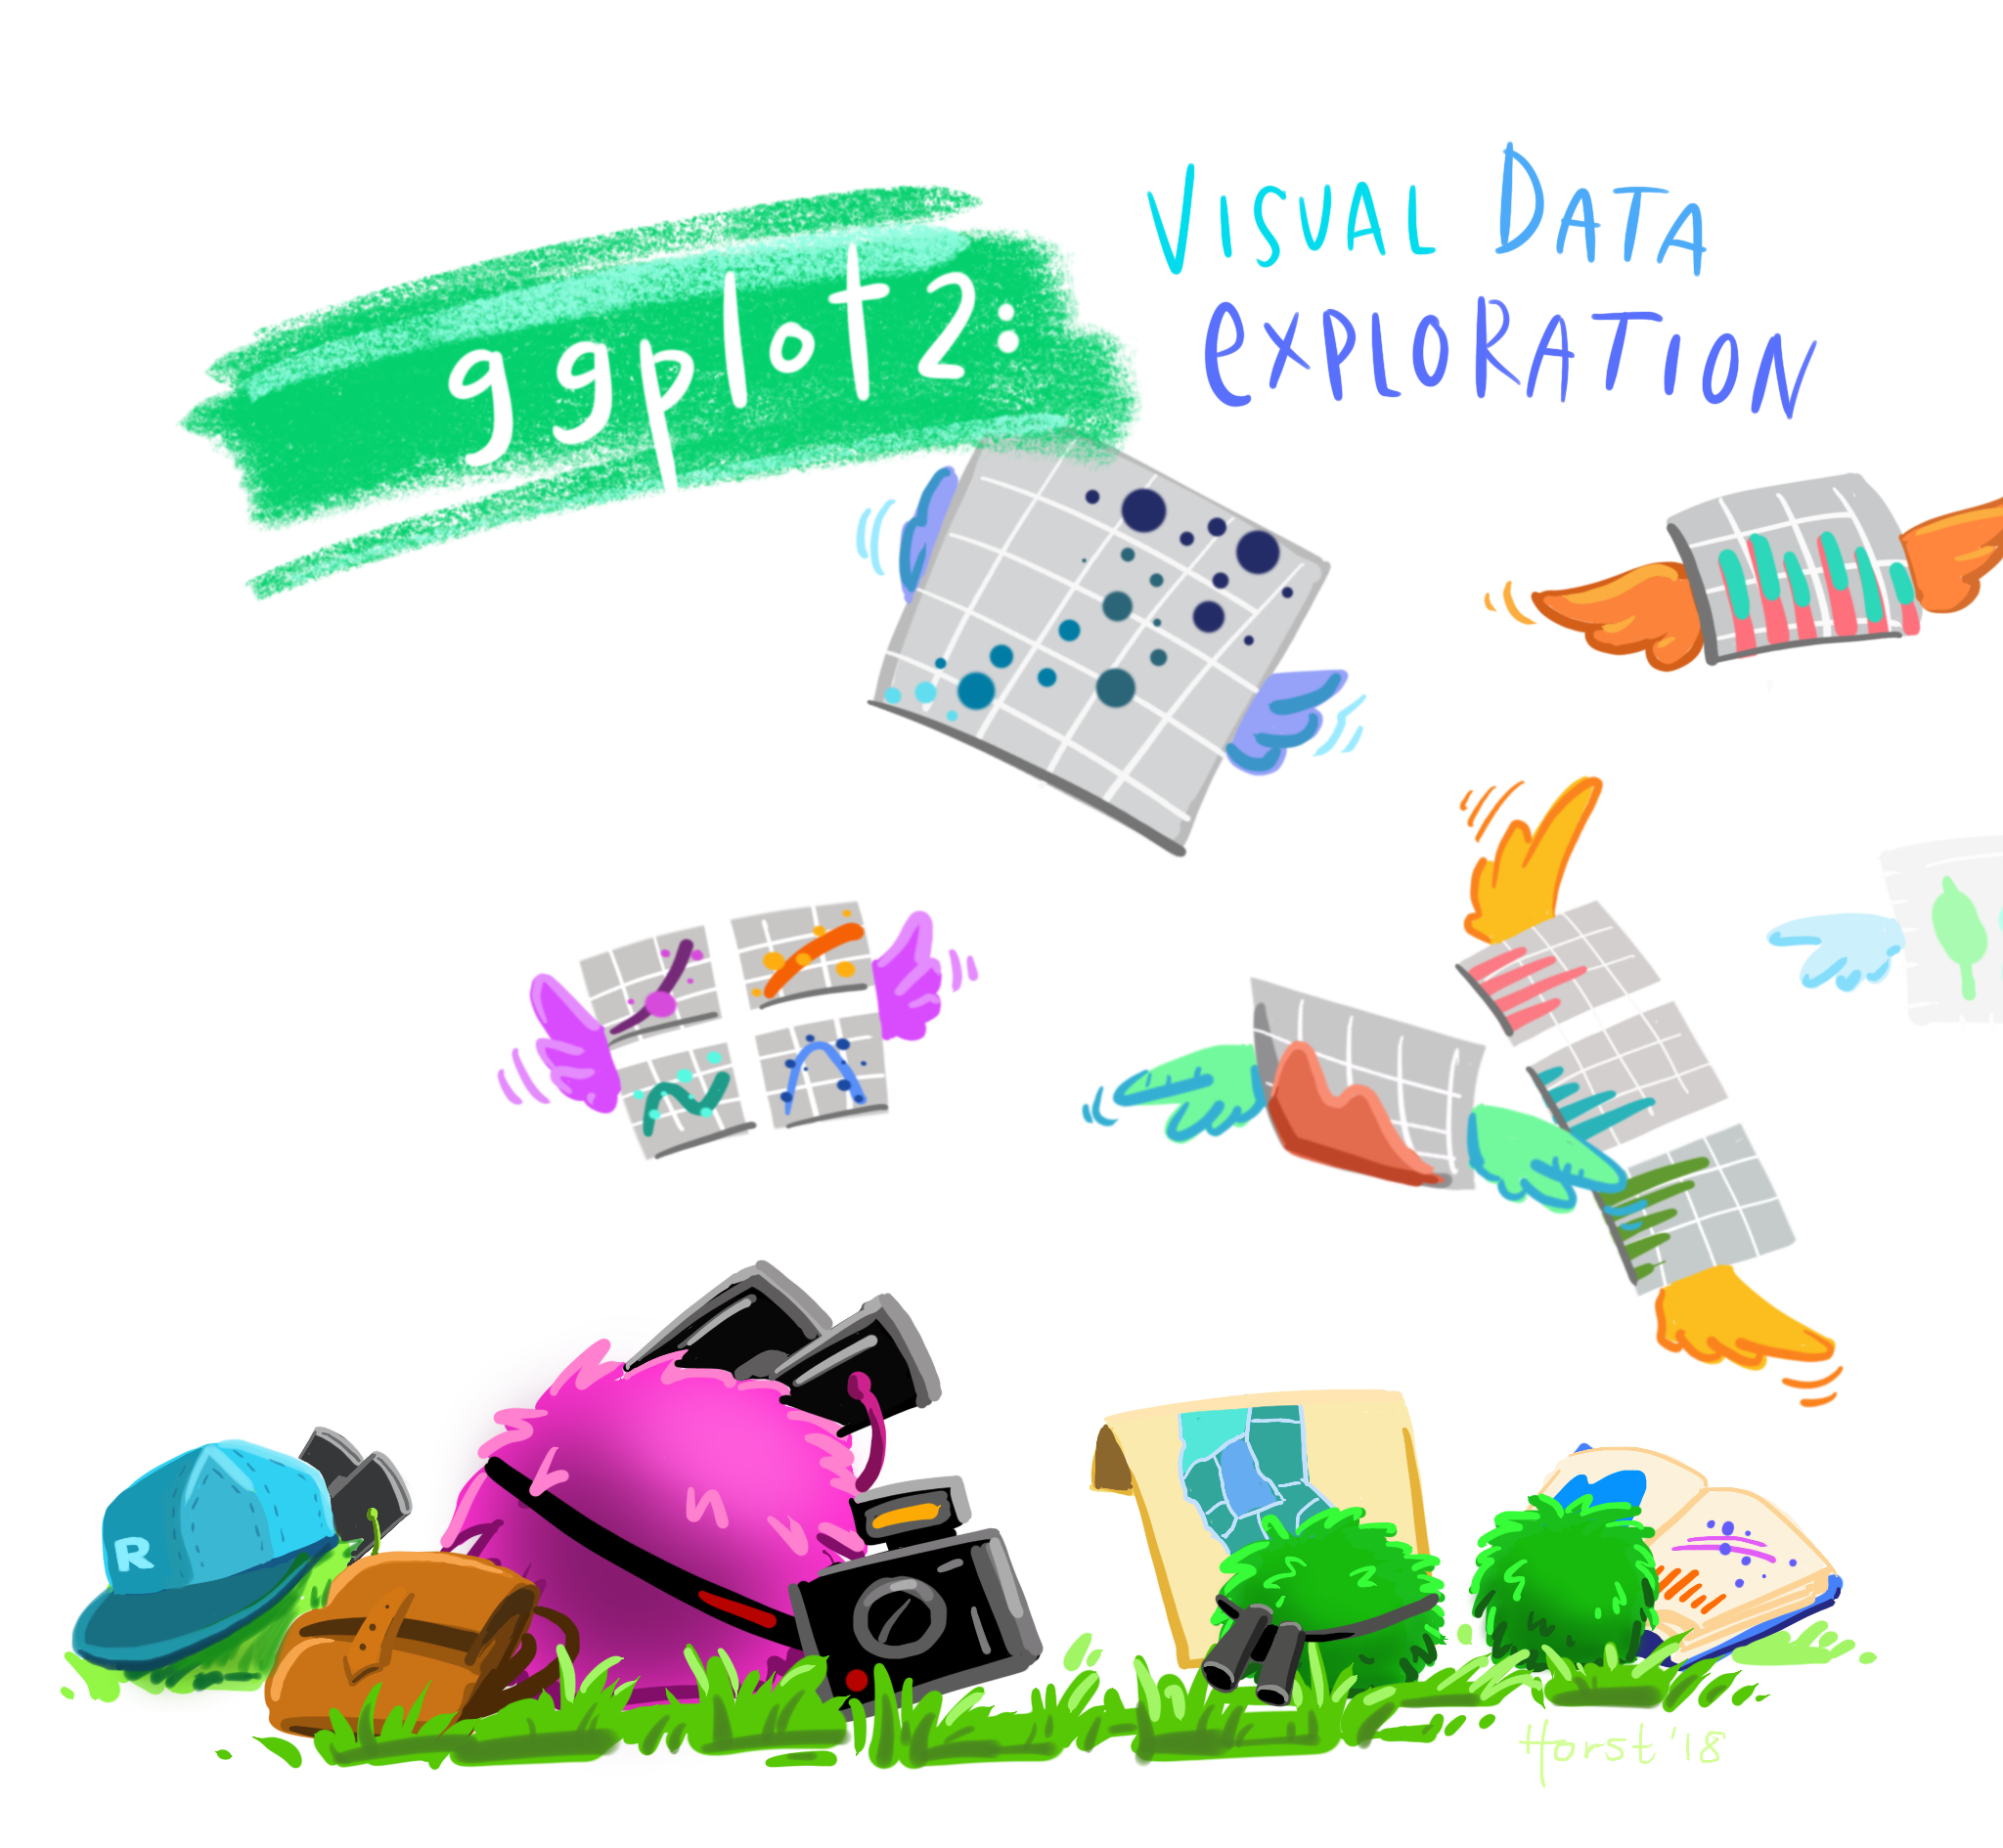
\includegraphics{assets/images/ggplot2_exploratory.png}
\caption{ggplot2}
\end{figure}

\hypertarget{learning-objectives-2}{%
\section{Learning Objectives}\label{learning-objectives-2}}

After completing this lab, you should be able to:

Install and load R packages.

Understand why data visualization is a useful tool for science communication.

Know and apply the APA guidelines for figures in APA manuscripts.

Understand the basic ``grammar of graphics'' used by \texttt{ggplot2}.

Apply the basic ``grammar of graphics'' to visualize data in R.

\hypertarget{prepare-for-the-lab-2}{%
\section{Prepare for the Lab}\label{prepare-for-the-lab-2}}

Ensure that you are comfortable with the content in labs 1 and 2.

\hypertarget{lab-activity-2}{%
\section{Lab Activity}\label{lab-activity-2}}

Use the \href{assets/data/anscombe_long.csv}{anscombe\_long.csv} data for this lab activity.

\hypertarget{setup}{%
\subsection{Setup}\label{setup}}

\begin{enumerate}
\def\labelenumi{\arabic{enumi}.}
\tightlist
\item
  If you haven't already, install \texttt{ggplot2}.
\item
  Load \texttt{ggplot2}.
\item
  Import \href{assets/data/anscombe_long.csv}{anscombe\_long.csv} into R as a \texttt{data.frame} named \texttt{anscombe\_long}.
\item
  Convert \texttt{anscombe\_long\$dataset} to a factor with levels: 1 = ``I'', 2 = ``II'', 3 = ``III'', and 4 = ``IV''.
\end{enumerate}

\hypertarget{plots}{%
\subsection{Plots}\label{plots}}

Write a script to produce each of the following plots. All of them use the \href{assets/data/anscombe_long.csv}{anscombe\_long.csv} data.

\hypertarget{plot-1-histograms}{%
\subsection{Plot 1: Histograms}\label{plot-1-histograms}}

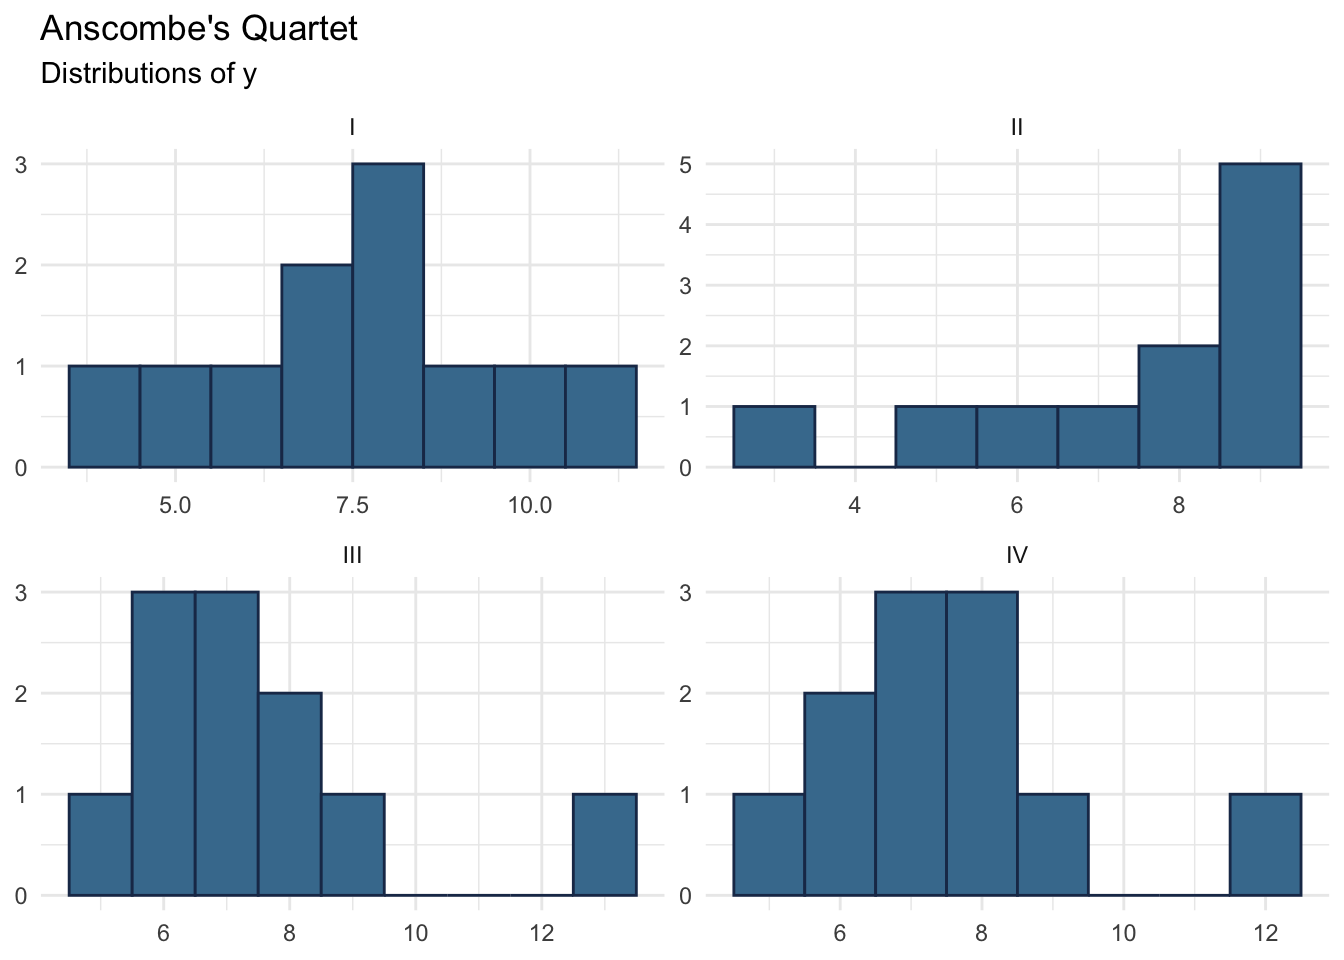
\includegraphics{03-data-viz_files/figure-latex/plot1-1.pdf}

\hypertarget{plot-2-boxplot}{%
\subsection{Plot 2: Boxplot}\label{plot-2-boxplot}}

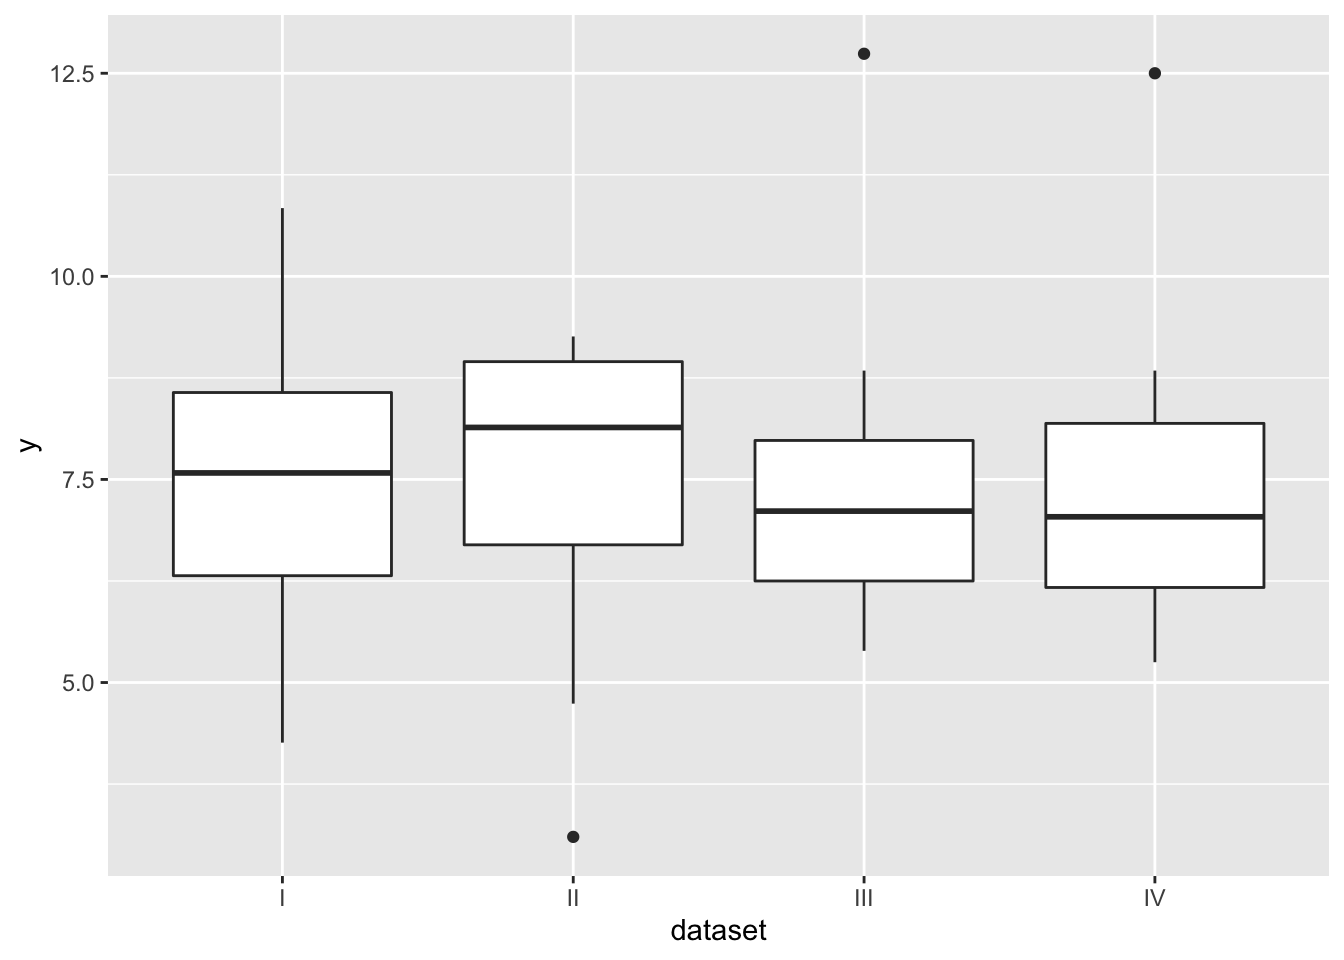
\includegraphics{03-data-viz_files/figure-latex/plot2-1.pdf}

\hypertarget{plot-3-scatter-plot}{%
\subsection{Plot 3: Scatter Plot}\label{plot-3-scatter-plot}}

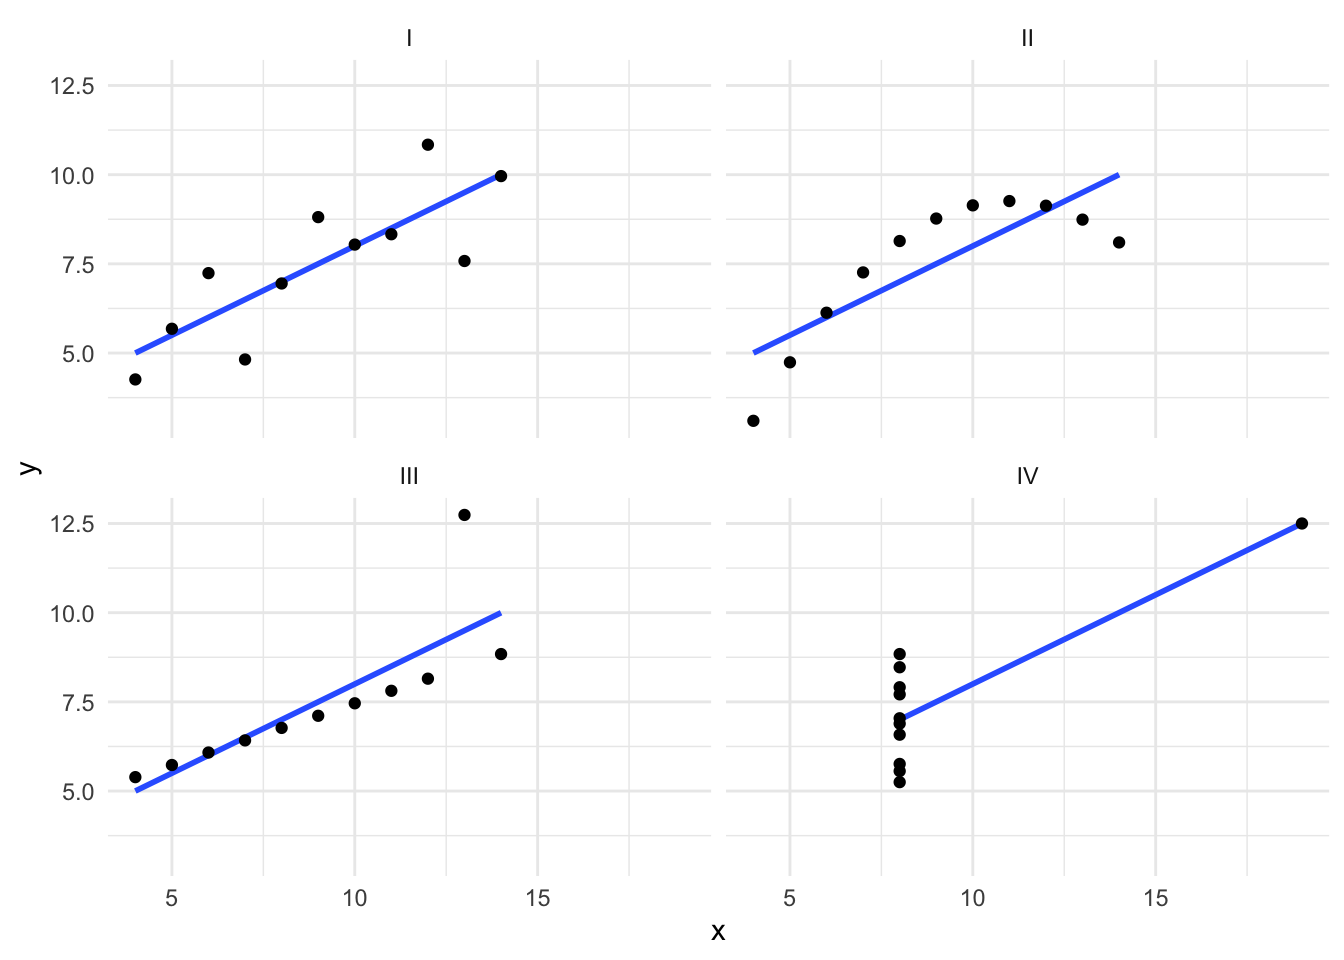
\includegraphics{03-data-viz_files/figure-latex/plot3-1.pdf}

\hypertarget{plot-4-jitter-plot}{%
\subsection{Plot 4: Jitter Plot}\label{plot-4-jitter-plot}}

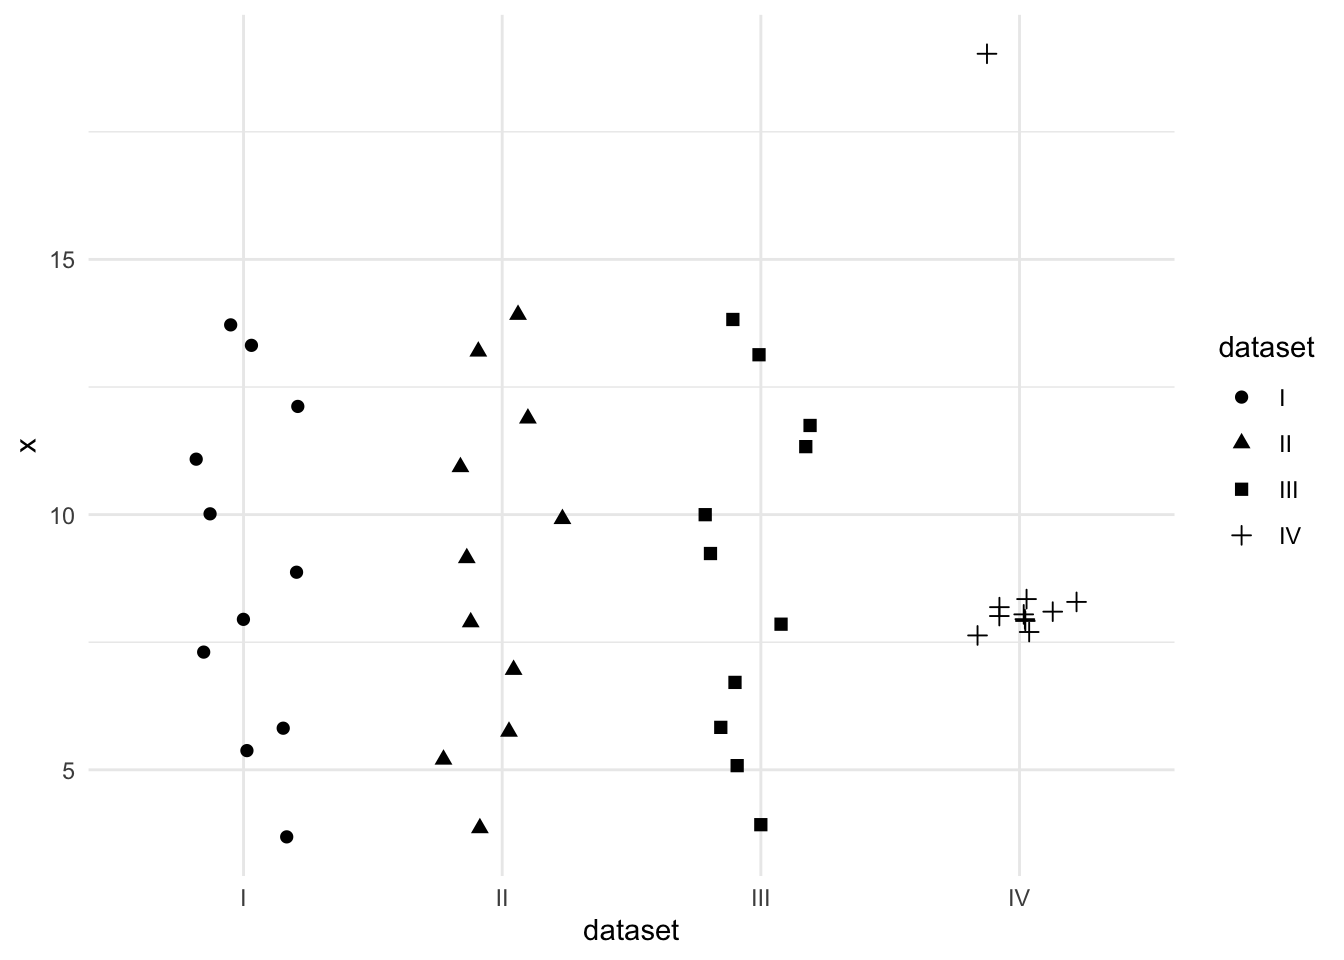
\includegraphics{03-data-viz_files/figure-latex/plot4-1.pdf}

\hypertarget{tips-for-recreating-plot-4}{%
\subsubsection*{Tips for Recreating Plot 4}\label{tips-for-recreating-plot-4}}
\addcontentsline{toc}{subsubsection}{Tips for Recreating Plot 4}

Identify the aesthetic mappings before you start.

\begin{itemize}
\tightlist
\item
  Which variable is mapped to x?
\item
  Which is mapped to y?
\item
  Are there any other aesthetic mappings?
\end{itemize}

Use \texttt{geom\_jitter()} to plot the points. \texttt{geom\_jitter()} is a variant of \texttt{geom\_point()} that adds a little\ldots{} jitter. It's useful when points would otherwise be overlapping. Note that the jitter is random, so your plot will not match this one exactly. The jitter can also affect the range of the scale axes.

Set the width of \texttt{geom\_jitter()} to be equal to 0.25.

This plot uses \texttt{theme\_minimal()}. You are free to use whatever theme you prefer.

\hypertarget{resources-1}{%
\section{Resources}\label{resources-1}}

\href{assets/slides/03-data-visualisation-slides.pdf}{Data Visualization Slides}

  \bibliography{book.bib,packages.bib}

\end{document}
